\documentclass[10pt]{article}         %% What type of document you're writing.

%%%%% Preamble

%% Packages to use
\usepackage{amsmath,amsfonts,amssymb,graphicx}   %% AMS mathematics macros
\usepackage[german]{babel}
\usepackage[utf8]{inputenc}
\usepackage{titlesec}

\setcounter{secnumdepth}{4}
\titleformat{\paragraph}
{\normalfont\normalsize\bfseries}{\theparagraph}{1em}{}
\titlespacing*{\paragraph}
{0pt}{3.25ex plus 1ex minus 0.2ex}{1.5ex plus 0.2ex}


%% Title Information.
\title{Optimierungsmethoden}
\author{Timon Tschanz, Pascal Zingg}
%% \date{}           %% By default, LaTeX uses the current date

%%%%% The Document

\begin{document}

\maketitle

\section{Einführung}
Im Rahmen des Kurses Analysis haben wir uns mit verschiednen Optimierungsaufgaben vertraut gemacht. Die grundlegende Technik, die wir dazu verwendeten, war die 1. Ableitung gleich 0 zu setzen, damit wir ein optimales Ergebnis für ein konkretes Problem erhielten. In diesem Bericht befassen wir uns näher mit Algorithmen, welche es ermöglichen Extremalstellen zu berechnen. Zudem diskutieren wir anhand von diversen Aufgabenstellungen, wie diese zur Anwendung kommen können. Durch diverse Visualisierungen versuchen wir mit diesem Bericht versuchen wir die Ergebnisse bildlich darzustellen, was aus unserer Sicht auch zu einer glaubwürdigeren Diskussion führen wird.

\section{Motivation}
Da es in unserer Umgebung sehr viele Problemstellungen gibt, bei denen jeweils ein Optimum gesucht ist, sehen wir in dieser Arbeit eine konkrete und relativ einfache Anwendung der Ableitungen. Die Algorithmen, welche wir mit Python umgsetzt haben, sind wiederverwendbar, da wir sie so weit als möglich versuchten, zu parametrisieren. 

\pagebreak
\section{Auswertungsverfahren}
\subsection{Algorithmen}
Um die Extremalstellen einer spezifischen Funktion zu errechnen, gibt es diverse Vorgehensweisen. In diesem Kapitel gehen wir auf die 3 im Unterricht behandelten Verfahren ein und erläutern ihre Funktionsweise. 

\subsubsection{Gradientenverfahren}
Durch diese Methode wird im generellen versucht, sich an eine Extremalstelle anzunähren. $x_0$ wird als Startpunkt definiert. Vorausgesetzt wird hierbei, dass sich der Punkt links von einer Extremalstelle befindet. Veranschaulichen wir uns die nachfolgende quadratische Funktion:
\[
    f(x)=x^2
\]

Abbildung X verdeutlicht anhand der quadratischen Funtkion das `Abtasten' und Annähern an eine Extremalstelle. Durch das festgesetzte Lambda wir die Granularität festgesetzt, also den Abstand zum vorangehenden Punkt. Dies hat natürlich Konsequenzen auf die Laufzeit unseres Algorithmus. Wir werden die Laufzeiten der verschiednen Verfahren in den nachfolgenden Kapitel gegenüberstellen und auswerten. 

\begin{figure}[!ht]
    \centering
    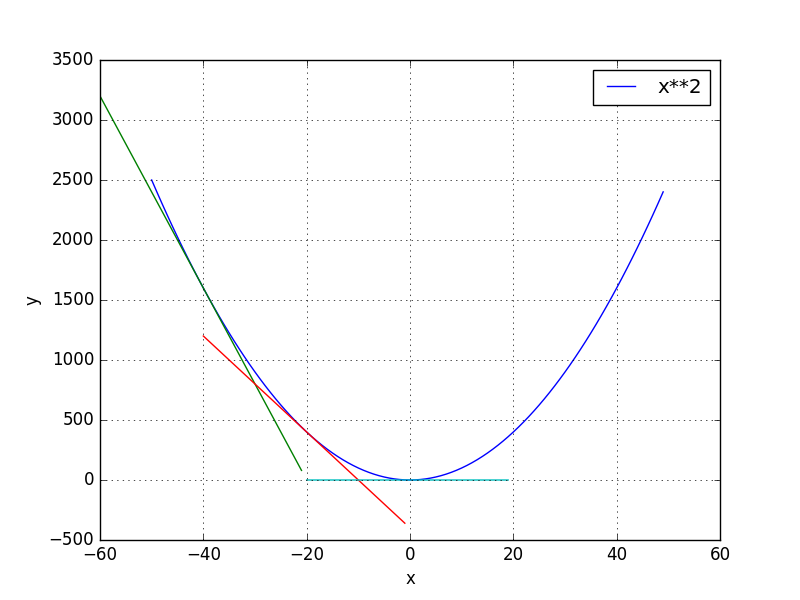
\includegraphics[width=0.9\textwidth]{gradient}
    \caption{Funktion $x^2$ mit Annäherung an Extremalstelle}\label{gradientx}
\end{figure}

\paragraph{Laufzeit}
Der Algorithmus läuft in $O(???)$

\paragraph{Bedingungen}
In Abbildung~\ref{gradientx} wird veranschaulicht, wie der Algorithmus funktioniert. Als Vorbedingung ist ein Startpunkt notwenig, welcher zwingend links von einer Extremalstelle liegt. Ausserdem muss mit diesem trivialen Algorithmus vorher sichergestellt werden, dass die Funktion überhaupt Extremalstellen besitzt, was ansosten zu einem unendlichen Loop führen kann. In unserem Beispiel mit der quadratischen Funktion $x^2$ wählen wir zum Beispiel den Punkt $x=-5$ aus. Wir können uns versichern, dass der Punkt links von einer Extremalstelle liegt und die Funktion überhaupt eine Extremalstelle besitzt. Natürlich ist diese von blossem Auge sofort erkennbar. 

\paragraph{Funktion von Lambda}
Der Algorithmus beginnt also vom Punkt $x=-5$ an, die 1. Ableitung zu berechnen. Hat er diese berechnet und ist diese ungleich 0, so wird mit Lambda ein neuer Punkt definiert, welcher sich etwas weiter Rechts auf der x-Achse befindet. Der Algorithmus ist so aufgebaut, dass er eine gewisse Genauigkeit aufweisen muss, um eine Extremalstelle eindeutig zu identifizieren. Diese Genauigkeit muss *unbedingt* kleiner sein als Lambda, da sonst die Stelle einfach übersprungen werden kann.

\subsubsection{Nelder-Mead}
TODO


\subsubsection{Nullstelle der Ableitung}
Durch den Bisektionsalgorithmus kann mithilfe der Ableitung eine Nullstelle, das heisst eine Extremalstelle ermittelt werden. Mithilfe eines anderen Algorithmus, in unserem Falle der Bisektionsalgorithmus, näheren wir uns ähnlich wie mit dem Gradientenverfahren an die Nullstelle an. 

\begin{figure}[!ht]
    \centering
    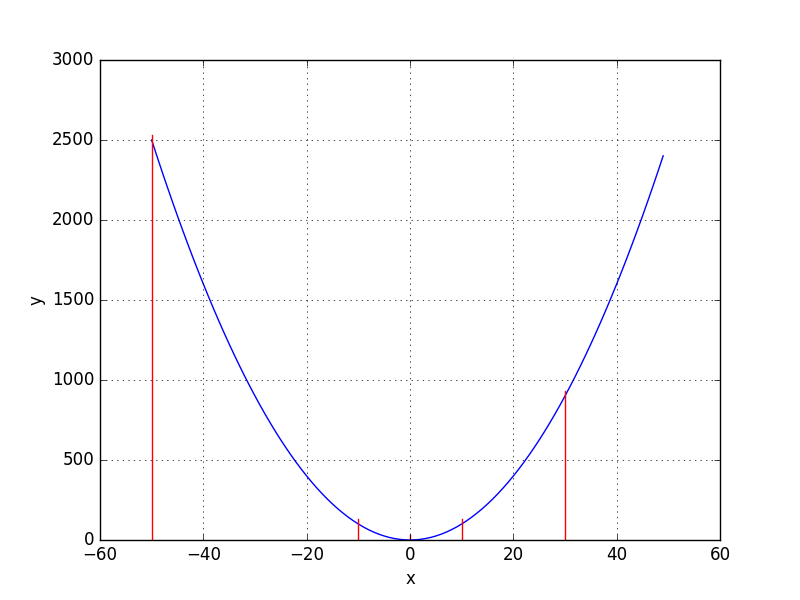
\includegraphics[width=0.9\textwidth]{bisektion}
    \caption{Bisektionsalgorithmus}\label{bisektion}
\end{figure}

Wie der Abbildung~\ref{bisektion} entnommen werden kann, schränkt sich der Bereich einr möglichen Nullstelle durch eine linke und rechte Schranke immer mehr ein.

\paragraph{Laufzeit}
Da der Bisektionsalgorithmus immer halbiert wird, das heisst die durchzusuchenden Wertebereiche logarithmisch schrumpfen, wird die Laufzeit vom Intervall $n=b-a$ gleich $O(\log(n))$ betragen. Die Berechnung der Ableitung wird hier wie bei den anderen Methoden ausser Acht gelassen. Wir können hierbei also feststellen, dass der Algorithmus effizient ist. Leider trübt dieser Vorteil, da er doch sehr eingeschränkt verwendet werden muss, was im nächsten Abschnitt näher erläutert wird.

\paragraph{Bedingungen}
Es muss vorgänig ein Intervall definiert werden, in welchem Extremalstellen anzutreffen sind. Unglücklicherweise kann bei zwei solchen Stellen nicht differenziert werden, dass sich tatsälich mehrere Stellen in dem Intervall befinden. Aus diesem Grund muss für unseren Algorithmus folgende Vorbedingung erfüllt werden: Der Intervall, welcher im Voraus definiert wird, darf nur genau eine Extremalstelle beinhalten. Wir haben uns Gedanken gemacht, wie wir dieses durchaus unschöne Problem lösen könnten. Man dürfte keine der ignorierten Seiten des Bisektionsalgorithmus ausser Acht lassen, da sich dort weitere Stellen befinden könnten. Dies würde den grundsätzlichen Nutzen des Bisektionsalgorithmus zerstören. Aus diesem Grund beschlossen wir, die Vorbedingung wie bereits erwähnt aufzustellen.

\pagebreak
\section{Anwendungsbeispiele}
\subsection{Der Rettungsschwimmer}
Ein Rettungsschwimmer will einer ertrinkenden Person im Wasser helfen. An Land rennt er mit $4.1 m/s$, im Wasser schwimmt er mit $2.1 m/s$. Welcher Weg an Land und im Wasser ist optimal, um in möglichst geringer Zeit zum Ertrinkenden zu gelangen? \\
    Diese Aufgabe klingt an sich trivial. Ein kleines Hindernis gibt es hierbei aber: Es sind keine Längenangaben vorhanden, was bedeutet, dass wir ein parametriesertes Ergebnis erwarten müssen. Abbildung~\ref{retts} zeigt, wie wir die Längen aufgeteilt haben.

\begin{figure}[!ht]
    \centering
    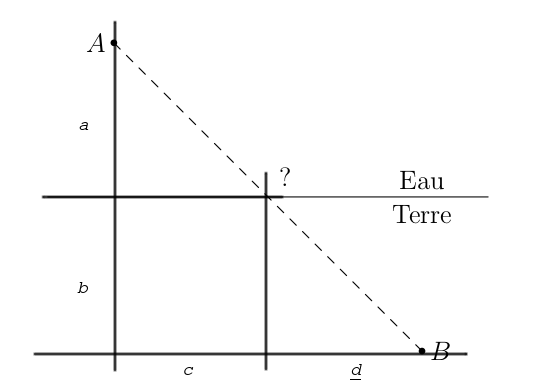
\includegraphics[width=0.9\textwidth]{rettungsschwimmer}
    \caption{Rettungsschwimmer}\label{retts}
\end{figure}

Da keine Längenangaben vorhanden sind, versuchten wir mittels verschiedenen Annahmen, uns an eine mögliche allgemeine Lösung für das Problem heranzutasten. Wie in~\ref{retts} eingezeichnet, gibt es die vier variablen Längen $a, b, c, d$. Kümmern wir uns zuerst um das Aufstellen einer Gleichung für das Optimierungsproblem. Uns ist bekannt, dass sich die Geschwindigkeit $v$ aus $s/t$ zusammensetzt. Des weiteren Wissen wir, nach was wir Optmimieren müssen: Der Zeit $t$. \\
Nach Pythagoras können wir auch die Längen berechnen, welche sich aus den Teilstrecken ergeben:
\begin{align}
    s_1=\sqrt{a^2+c^2} \\
    s_2=\sqrt{b^2+d^2}
\end{align}

Uns liegt nun auch auf der Hand, wie wir die Gleichung aufstellen müssen, um nach der Zeit zu optimieren. Allgemein lassen sich Optimierungsprobleme lösen, in dem die Ableitung der Gleichung gleich 0 gesetzt wird und nach einer gewünschten Variable aufgelöst wird. Wir beginnen zunächst, die Gleichung zusammenzusetzen. Um die optimale Zeit zu erhalten, müssen wir versuchen, die Summe der Zeit während des Laufens und die Zeit wärend des Schwimmens in Form einer Gleichung darzustellen. Da die Geschwindigkeit der jeweiligen Teilstrecken bekannt ist, kann dafür jeweils $s/v$ verwendet werden. Das sieht dann folgendermassen aus:

\begin{align}
    t = \frac{s_1}{2.1} + \frac{s_2}{4.1}
\end{align}

Setzen wir nun $s_1$ und $s_2$ in die Gleichung ein, erhalten wir:

\begin{align}
    t = \frac{\sqrt{a^2+c^2}}{2.1} + \frac{\sqrt{b^2+d^2}}{4.1}
\end{align}

Somit haben wir eine Gleichung gefunden, welche unser Problem zusammenfasst. Jedoch ist ersichtlich, dass wir nicht nur x als Variable haben, sondern gleich 4 unbekannte. Wir nähern uns an das Problem heran, indem wir nun Annahmen treffen, wie die Strecken zueinander stehen. \\
Der einfachste Fall liegt auf der Hand: Wir nehmen an, dass sich Punkt A und Punkt B gleich weit weg vom Ufer befinden, also $a=b$. Ausserdem gehen wir davon aus, dass $c+d=a+b$ ergibt. Mit diesen Annahmen ergibt sich folgende Gleichung für die Ableitung:

\begin{align}
    \frac{df}{dx}(\frac{\sqrt{m^2+{(2m-x)}^2}}{2.1} + \frac{\sqrt{m^2+x^2}}{4.1})
\end{align}

Wir haben nun $m$ verwendet, welches sowohl $a$ und $b$ repräsentiert. $x$ dient als Strecke $d$. Die 1. Ableitung ergibt:

\begin{align}
    \frac{0.243902x}{\sqrt{m^2+x^2}}+\frac{0.47619(2m-x)}{\sqrt{m^2+{2m-x}^2}}
\end{align}

Setzen wir Gleichung (6) zu 0 und lösen nach $x$ auf, erhalten wir als Resultat:
\[
    x = 1.5259m
\]

$m$ können wir nun frei wählen. Folgende Grafik veranschaulicht das Optimum, falls wir $m=100$ wählen:

\pagebreak
\begin{figure}[!ht]
    \centering
    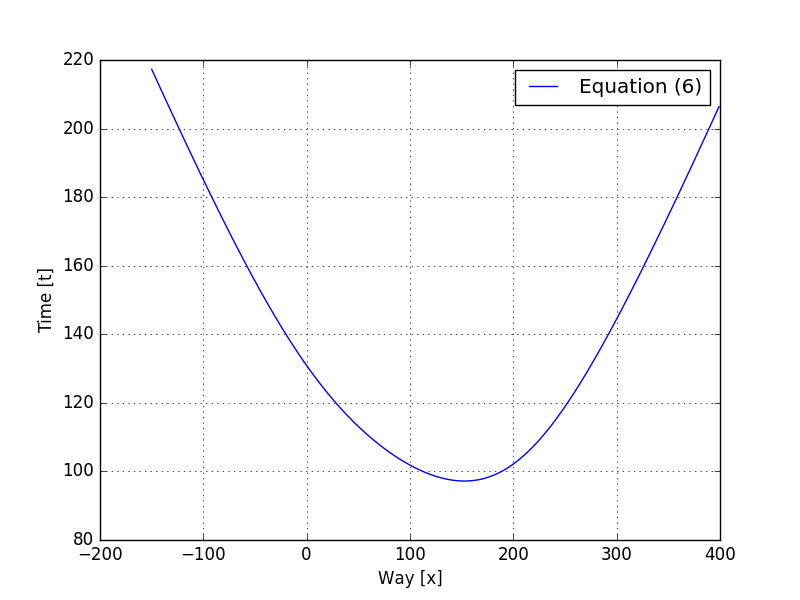
\includegraphics[width=0.9\textwidth]{lifeguard_100}
    \caption{Rettungsschwimmer mit $m=100$}\label{lifeguard_100}
\end{figure}

Es ist ersichtlich, dass bei $y=0$ der Wert von $x$ bei $1.5259*100=152.59$ liegt.


\subsection{Versicherungsprämienrechner}

\section{Diskussion}
\subsubsection{Anwendbarkeit der Methoden}
\subsubsection{Vorteile}
\subsubsection{Nachteile}
\subsubsection{Gegenüberstellung der Laufzeiten}

\end{document}
